\chapter{L'esperimento di Rutherford}
\section{Thomson vs Rutherford : chi ha ragione?}
Nei primi anni del 900 vi erano due modelli atomici : 
\begin{itemize}
        \item Il \textbf{modello di Thomson} per il quale l'atomo e schematizzato come una sfera
                con densità di carica uniforme, sostanzialmente le cariche positive e 
                negative erano distribuite uniformemente.
        \item il \textbf{modello di Rutherford} l'atomo era costituito da un nucleo puntiforme
                carico positivamente al centro e le cariche negative che gli orbitavano attorno.
\end{itemize}
Nel caso del modello di Thomson il campo elettrico dovuto dalle cariche, per il teorema di 
Gauss è dato da:
\begin{figure}[!h]
    \centering
    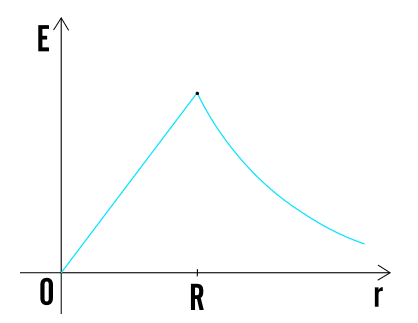
\includegraphics[scale=0.5]{ch5Ratherford/CampoE}
\end{figure}

Per capire come una particelle varia la direzione della quantità di moto, dobbiamo integrare
nel tempo la forza dovuta dal campo elettrico, integrale molto difficile, ciò che possiamo fare però è fare una maggiorazione poichè a noi interessa
la massima deflessione che la particella può subire.\\
$F_{max}$ per $r=R$ è:
\begin{align*}
    F_{max} = \frac{Ze\rho R}{3\epsilon_{0}}
\end{align*}
Essa si collega alla deflessione subita dalla particella dalla seguente:
\begin{align*}
        \theta_{max} = \frac{\Delta P}{P_{i}} = \frac{F_{max}\Delta t_{max}}{mv_{0}}
\end{align*}
Considerando il mezzo come una lamina d'oro e energia della particella di circa 5MeV si 
ottiene che la massima deflessione è :
\begin{align*}
    \theta_{max} \sim 3\cross10^{-4}rad
\end{align*}
Nello strato di oro che considereremo per l'esperimento di Rutherford si hanno circa 2000 atomi, 
essendo le deflessioni completamente casuali, considerando il processo come un Random Walk :
\begin{align*}
    \theta_{f} = \sqrt{2000}\theta_{max} \sim 1,3\cross10^{-2}rad
\end{align*}
Viene fuori che l'angolo massimo di deflessione che ci aspettiamo nel caso di uno scattering 
di una particella carica con un atomo descritto dal modello di Thomson è minuscolo, circa 
1 grado
\section{L'esperimento di Rutherford nella pratica}
Rutherford propose un modello atomico nel quale tutte le cariche positive sono concentrate 
in un piccolo volume al centro dell'atomo e le cariche negative orbitavano attorno ad esso.
L'esperimento che fece per provare ciò consisteva nel colpire tali atomi con particelle 
$\alpha$ le quali, entrando nel volume dell'atomo non sentiranno l'influenza del campo elettrico 
degli elettroni ( che per il teorema di Gauss è nullo ).
L'interazione fra le particelle $\alpha$ e il nucleo sarà trattato con metodi di meccanica 
classica e schematizzato come segue.
\begin{figure}[!h]
    \centering
    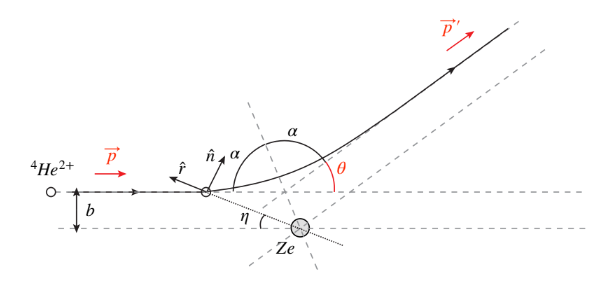
\includegraphics[scale=0.5]{ch5Ratherford/Rutherford}
    \caption{Tratiettoria della particella $\alpha$ deviata dal potenziale coulombiano del nucleo}
\end{figure}

dove : 
\begin{itemize}
        \item b = prametro di impatto; 
        \item $\theta$ = angolo di deflessione;
        \item \textit{z}e = carica particella $\alpha$; 
        \item Ze = nucleo bersaglio.
\end{itemize}
Ciò che vogliamo trovare è la relazione che intercorre fra il parametro di impatto e l'angolo
di diffusione, il fatto che trattiamo tale problema con metodi classici è molto importante 
perchè rende il problema \textbf{completamente deterministico}. \\
\begin{tcolorbox}[colback=red!5!white,colframe=red!50!black,title=ATTENZIONE !]
Perchè possiamo trattare il problema con metodi classici e non relativistici ? \\
In quegli anni non esistevano gli acceleratori di particelle, l'unica fonte erano quindi le radiazioni
che però producono proiettili con energia cinetica $T \sim 5MeV$ molto più piccola della massa della 
particella $\alpha$ che invece si aggira sui 4 GeV
\end{tcolorbox}
\newpage
La particella $\alpha$ subirà una forza repulsiva diretta radialmente :
\begin{align*}
    \va{F} = \frac{\textit{z}Ze^2}{4\pi \epsilon_{0}r^2}\vu{r}
\end{align*}
\begin{tcolorbox}[colback=red!5!white,colframe=red!50!black,title=ATTENZIONE !]
Il fatto che la forza sia centrale è molto importante poichè ci dice che la velocità non 
cambia se non in direzione, possiamo quindi applicare la conservazione del momento quantità 
di moto !
\end{tcolorbox}
Applichiamo la conservazione del momento quantità di moto : 
\begin{align*}
        \va{L} &= m_{\alpha}r^2\dv{\beta}{t} \\ 
        \va{L_{i}} &= m_{\alpha}bv_{0} 
\end{align*}
eguagliando si ottiene : 
\begin{align*}
    \frac{1}{r^2} = \frac{1}{bv_{0}}\dv{\beta}{t}
\end{align*}
Scriviamo ora l'equazione del moto \textbf{lungo l'asse y} : 
\begin{align*}
        m_{\alpha}\dv{v_{y}}{t} &= \frac{\textit{z}Ze^2}{4\pi\epsilon_{0}r^2}\sin{\beta} \\
        m_{\alpha}\dv{v_{y}}{t} &= \frac{\textit{z}Ze^2}{4\pi\epsilon_{0}bv_{0}}\sin{\beta}\dv{\beta}{t}
\end{align*}
Considerando due istanti A(t = -$\infty$) e B(t = $\infty$) : 
\begin{align*}
    v_{y}(A) = 0  & \quad  v_{y}(B) = v_{0}\sin{\theta} \\
    \beta(A) = 0  & \quad  \beta(B) = \pi - \theta 
\end{align*}
otteniamo : 
\begin{align*}
        \int_{0}^{v_{0}\sin{\theta}}\dd{v_{y}} = \frac{\textit{z}Ze^2}{4\pi\epsilon_{0}bv_{0}}\int_{0}^{\pi - \theta}\sin{\beta}\dd{\beta}
\end{align*}
finalmente arriviamo al risultato che volevamo ottenere all'inizio : 
\begin{align*}
        &v_{0}\sin{\theta} = \frac{\textit{z}Ze^2}{4\pi\epsilon_{0}bv_{0}}\qty[-\cos{\pi - \theta} + 1] \\[1em]
        &b = \frac{\textit{z}Ze^2}{4\pi\epsilon_{0}v_{0}^2}\frac{1 + \cos{\theta}}{\sin{\theta}} 
\end{align*}
\newpage
\begin{tcolorbox}[colback=red!5!white,colframe=red!50!black,title=ATTENZIONE !]
\begin{align*}
        b = \frac{\textit{z}Ze^2}{4\pi\epsilon_{0}bv_{0}}\cot{\frac{\theta}{2}}
\end{align*}
\end{tcolorbox}
\section{La sezione d'urto differenziale}
In un esperimento non si conosce il parametro di impatto della particella, non si può quindi
dato un determinato valore di b a quale valore di $\theta$ corrisponde, ma qualcosa possiamo fare ossia 
ricavarci la distribuzione di probabilità del parametro b considerando che possa essere distribuito 
lungo un anello centrato all'intorno della posizione del bersaglio.
\begin{figure}[!h]
    \centering
    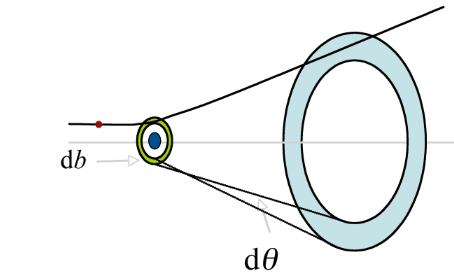
\includegraphics[scale=0.8]{ch5Ratherford/distribuzioneB}
\end{figure}

\begin{align*}
    &P(b)\dd{b} = \frac{2\pi b\dd{b}}{\pi R^2} \\[1em]
    &b = k\frac{1}{2}\cot{\frac{\theta}{2}} \quad \dd{b} = \frac{k}{2}\frac{\dd{\theta}}{2}\frac{1}{\sin^2{\theta/2}} \\[1em]
    &P(\Omega)\dd{\Omega} = \frac{\textit{z}Ze^2}{4\pi\epsilon_{0}bv_{0}}\frac{\dd{\Omega}}{16\sin^4{\theta/2}}\frac{1}{R^2\pi}
\end{align*}

$P(\Theta)$ non è altro che la probabilità dell'angolo soldo, essa è tanto più alta quando l'angolo di diffusione è basso, 
ma, ricordandoci che la sezione d'urto non è altro che la probabilità di un processo allora : 
\begin{align*}
        \dv{\sigma}{\Omega} = \frac{\textit{z}Ze^2}{4\pi\epsilon_{0}bv_{0}}\frac{1}{16\sin^4{\theta/2}}
\end{align*}
